\begin{singlespace}
    \chapter{\textbf{Appendix C: Supplemental material for "The relative cost of resource use for photosynthesis drives variance in leaf nitrogen content across a climate and soil resource availability gradient"}}
\end{singlespace}

\setcounter{table}{0}
\renewcommand{\thetable}{C\arabic{table}}

\setcounter{figure}{0}
\renewcommand{\thefigure}{C\arabic{figure}}


\section*{C.1 Calculations for soil water holding capacity}\label{appendix.c1}
\noindent Water holding capacity ($\theta_\mathrm{WHC}$; mm) was calculated as a function of the volumetric soil water storage at field capacity ($W_\mathrm{FC}$; $\mathrm{m^3\ m^{-3}}$), and the volumetric soil water storage at wilting point ($W_\mathrm{PWP}$; $\mathrm{m^3\ m^{-3}}$):

\begin{equation}
    \label{eqn_s4.1} \tag{C4.1}
    \theta_{WHC} = (W_{FC}-W_{PWP})(1-f_{gravel}) * min(z_{bedrock}, z_{max})
\end{equation}

\noindent where $f_\mathrm{gravel}$ (\%) is the fraction of gravel content in soil, $z_\mathrm{bedrock}$ (mm) is the distance to bedrock, and $z_\mathrm{max}$ (mm) is the maximum allowable distance to bedrock, set to 2000 mm. $W_\mathrm{FC}$ is calculated as:

\begin{equation}
    \label{eqn_s4.2} \tag{C4.2}
    \theta_{FC} = k_{fc}+(1.283*(k_{fc})^2-0.374*k_{fc}-0.015)
\end{equation}

\noindent where

\begin{equation}
    \label{eqn_s4.3} \tag{C4.3}
    \begin{aligned}
        k_{fc}= -0.251 * f_{sand} + 0.195 * f_{clay} + 0.011 * f_{OM} \\ + 0.006 * (f_{sand} * f_{OM}) - 0.027 * (f_{clay} \\ * f_{OM}) + 0.452 * (f_{sand} * f_{clay}) + 0.299
    \end{aligned}	
\end{equation}

\noindent $W_\mathrm{PWP}$ is calculated as:

\begin{equation}
    \label{eqn_s4.4} \tag{C4.4}
    W_{PWP}=k_{pwp}+(0.14*k_{pwp}-0.02)	
\end{equation}

\noindent where

\begin{equation}
    \label{eqn_s4.5} \tag{C4.5}
    \begin{aligned}
        k_{pwp} = -0.024 * f_{sand} + 0.487 * f_{clay} + 0.006 * f_{OM} \\ + 0.005 * (f_{sand} * f_{OM}) - 0.013 * (f_{clay} \\ * f_{OM}) + 0.068 * (f_{sand} * f_{clay}) + 0.031
    \end{aligned}
\end{equation}

\noindent In Equations \ref{eqn_s4.4} and \ref{eqn_s4.5}, $f_\mathrm{sand}$ (\%) is the fraction of sand content in soil (\%), $f_\mathrm{clay}$ (\%) is the fraction of clay content in soil (\%), and $f_\mathrm{OM}$ is the fraction of organic matter in soil (\%). Organic matter in the soil was calculated by converting soil organic carbon data extracted from SoilGrids 2.0 to soil organic matter using the van Bemmelen factor (1.724 conversion factor).
\clearpage


\begin{landscape}
    \begin{table}[]
        \caption{List of sampled species and their plant functional group assignment}
        \label{tab:tab.c1}
        \resizebox{\columnwidth}{!}{%
            \begin{tabular}{p{2cm}p{5cm}p{2cm}p{2cm}p{2cm}p{2cm}p{3.5cm}p{2cm}}
            \hline
            \textbf{Symbol} & \textbf{Species} & \textbf{\begin{tabular}[c]{@{}l@{}}Photo.\\ pathway\end{tabular}} &
            \textbf{\begin{tabular}[c]{@{}l@{}}Growth\\ duration\end{tabular}} & \textbf{Growth  habit} &
            \textbf{N-fixer?} & \textbf{\begin{tabular}[c]{@{}l@{}}Plant functional \\ group\end{tabular}} &
            \multicolumn{1}{l}{\textbf{\begin{tabular}[c]{@{}l@{}}Number \\ sampled\end{tabular}}} \\
            \hline
            ACAN11 & \textit{Acaciella angustissima}    & c3 & perennial & forb           & yes & c3\_N-fixer    & 3  \\
            AMAR2  & \textit{Ambrosia artemisiifolia}   & c3 & annual    & forb           & no  & c3\_non-fixer & 25 \\
            AMPS   & \textit{Ambrosia psilostachya}     & c3 & perennial & forb           & no  & c3\_non-fixer & 32 \\
            ARAL3  & \textit{Argemone albiflora}        & c3 & annual    & forb           & no  & c3\_non-fixer & 3  \\
            ARPU9  & \textit{Aristida purpurea}         & c4 & perennial & graminoid      & no  & c4\_non-fixer & 2  \\
            ASAS   & \textit{Asclepias asperula}        & c3 & perennial & forb           & no  & c3\_non-fixer & 3  \\
            ASLA4  & \textit{Asclepias latifolia}       & c3 & perennial & forb           & no  & c3\_non-fixer & 3  \\
            ASSY   & \textit{Asclepias syriaca}         & c3 & perennial & forb           & no  & c3\_non-fixer & 18 \\
            BOIS   & \textit{Bothriochloa ischaemum}    & c4 & perennial & graminoid      & no  & c4\_non-fixer & 6  \\
            BOSA   & \textit{Bothriochloa saccharoides} & c4 & perennial & graminoid      & no  & c4\_non-fixer & 6  \\
            CAPL3  & \textit{Carex planostachys}        & c4 & perennial & graminoid      & no  & c4\_non-fixer & 3  \\
            CAREX  & \textit{Carex} spp.                & c4 & perennial & graminoid      & no  & c4\_non-fixer & 16 \\
            CHFE3  & \textit{Chamaesyce fendleri}       & c3 & perennial & forb           & no  & c3\_non-fixer & 2  \\
            CHPI8  & \textit{Chyrysopsis pilosa}        & c3 & annual    & forb           & no  & c3\_non-fixer & 3  \\
            COCO13 & \textit{Conoclinium coelestinum}   & c3 & perennial & forb           & no  & c3\_non-fixer & 3  \\
            COER   & \textit{Commelina erecta}          & c3 & perennial & forb           & no  & c3\_non-fixer & 3  \\
            CRGLL  & \textit{Croton glandulosus}        & c3 & annual    & forb           & no  & c3\_non-fixer & 22 \\
            CYDA   & \textit{Cynodon dactylon}          & c4 & perennial & graminoid      & no  & c4\_non-fixer & 15 \\
            DIAN   & \textit{Dichanthium annulatum}     & c4 & perennial & graminoid      & no  & c4\_non-fixer & 8  \\
            ENPE4  & \textit{Engelmannia peristenia}    & c3 & perennial & forb           & no  & c3\_non-fixer & 6  \\
            EUMA8  & \textit{Euphorbia marginata}       & c3 & annual    & forb           & no  & c3\_non-fixer & 6  \\
            GAPU   & \textit{Gaillardia pulchella}      & c3 & annual    & forb           & no  & c3\_non-fixer & 16 \\
            GLGO   & \textit{Glandularia gooddingii}    & c3 & perennial & forb           & no  & c3\_non-fixer & 2  \\
            HEAN3  & \textit{Helianthus annuus}         & c3 & annual    & forb           & no  & c3\_non-fixer & 6  \\
            \hline
        \end{tabular}}
    \end{table}
\end{landscape}
\clearpage

\newpage
\begin{landscape}
    \begin{table}[]
        \caption{List of sampled species and their plant functional group assignment (cont.)}
        \label{tab:tab.c2}
        \resizebox{\columnwidth}{!}{%
            \begin{tabular}{p{2cm}p{5cm}p{2cm}p{2cm}p{2cm}p{2cm}p{3.5cm}p{2cm}}
        \hline
        \textbf{Symbol} & \textbf{Species} & \textbf{\begin{tabular}[c]{@{}l@{}}Photo.\\ pathway\end{tabular}} &
        \textbf{\begin{tabular}[c]{@{}l@{}}Growth\\ duration\end{tabular}} & \textbf{Growth habit} &
        \textbf{N-fixer?} & \textbf{\begin{tabular}[c]{@{}l@{}}Plant functional \\ group\end{tabular}} &
        \multicolumn{1}{l}{\textbf{\begin{tabular}[c]{@{}l@{}}Number \\ sampled\end{tabular}}} \\
        \hline
        HECA8  & \textit{Heterotheca canescens}     & c3 & perennial & forb           & no  & c3\_non-fixer & 2  \\
        HETE3  & \textit{Heliotropium tenellum}     & c3 & annual    & forb           & no  & c3\_non-fixer & 3  \\
        IVAX   & \textit{Iva axillaris}             & c3 & perennial & forb           & no  & c3\_non-fixer & 4  \\
        LIAT   & \textit{Lilaeopsis attenuata}      & c3 & perennial & forb           & no  & c3\_non-fixer & 3  \\
        LIPU   & \textit{Liatris punctata}          & c3 & perennial & forb           & no  & c3\_non-fixer & 3  \\
        LOPE   & \textit{Lolium perenne}            & c3 & perennial & graminoid      & no  & c3\_non-fixer & 9  \\
        MIQU2  & \textit{Mimosa quadrivalvis}       & c3 & perennial & forb           & yes & c3\_N-fixer    & 15 \\
        NALE3  & \textit{Nassella leucotricha}      & c3 & perennial & graminoid      & no  & c3\_non-fixer & 19 \\
        OECU2  & \textit{Oenothera curtiflora}      & c3 & annual    & forb           & no  & c3\_non-fixer & 3  \\
        OENOT  & \textit{Oenothera} spp.            & c3 & annual    & forb           & no  & c3\_non-fixer & 1  \\
        PAVI2  & \textit{Panicum virgatum}          & c4 & perennial & graminoid      & no  & c4\_non-fixer & 12 \\
        RACO3  & \textit{Ratibida columnifera}      & c3 & perennial & forb           & no  & c3\_non-fixer & 40 \\
        RHSET  & \textit{Rhynchosia senna}          & c3 & perennial & forb           & yes & c3\_N-fixer    & 1  \\
        RUHI2  & \textit{Rudbeckia hirta}           & c3 & perennial & forb           & no  & c3\_non-fixer & 3  \\
        RUNU   & \textit{Ruellia nudiflora}         & c3 & perennial & forb           & no  & c3\_non-fixer & 15 \\
        RUTR   & \textit{Rubus trivialis}           & c3 & perennial & vine           & no  & c3\_non-fixer & 3  \\
        SAFA2  & \textit{Salvia farinacea}          & c3 & perennial & forb           & no  & c3\_non-fixer & 7  \\
        SCHIZ4 & \textit{Schizachyrium} spp.        & c4 & perennial & graminoid      & no  & c4\_non-fixer & 8  \\
        SCSC   & \textit{Schizachyrium scoparium}   & c4 & perennial & graminoid      & no  & c4\_non-fixer & 3  \\
        SODI   & \textit{Solanum dimidiatum}        & c3 & perennial & forb           & no  & c3\_non-fixer & 1  \\
        SOEL   & \textit{Solanum elaeagnifolium}    & c3 & perennial & forb           & no  & c3\_non-fixer & 53 \\
        SOHA   & \textit{Sorghum halapense}         & c4 & perennial & graminoid      & no  & c4\_non-fixer & 38 \\
        STTE3  & \textit{Stillingia texana}         & c3 & perennial & forb           & no  & c3\_non-fixer & 3  \\
        VEOC   & \textit{Verbesina occidentalis}    & c3 & perennial & forb           & no  & c3\_non-fixer & 3  \\
        VEST   & \textit{Verbena stricta}           & c3 & perennial & forb           & no  & c3\_non-fixer & 3  \\
        \hline
    \end{tabular}}
\end{table}
\end{landscape}
\clearpage

\newpage
\begin{table}
    \centering
    \caption[Model selection results for soil moisture and vapor pressure deficit]{Model selection results for soil moisture and vapor pressure deficit. Soil moisture was used in a bivariate regression against log-transformed $\beta$, while vapor pressure deficit was used in bivariate regressions against leaf $C_\mathrm{i}$:$C_\mathrm{a}$}
    \label{tab:tab.c4}
    %\resizebox{\columnwidth}{!}{%
        \begin{tabular}{p{2cm}p{2cm}p{2cm}p{2cm}p{2cm}}
            & \multicolumn{2}{l}{Soil moisture} & \multicolumn{2}{l}{VPD} \\
            \hline
            Day & AICc              & RMSE              & AICc              & RMSE   \\
            \hline
            1  & 1870.80            & 1.4147            & -848.01           & 0.0738 \\
            2  & 1870.12            & 1.4136            & -847.68           & 0.0738 \\
            3  & \textbf{1870.10}   & \textbf{1.4135}   & -847.48           & 0.0738 \\
            4  & 1870.37            & 1.4141            & \textbf{-867.19}  & \textbf{0.0725} \\
            5  & 1870.76            & 1.4148            & -847.10           & 0.0738 \\
            6  & 1870.99            & 1.4153            & -847.00           & 0.0738 \\
            7  & 1871.26            & 1.4158            & -846.90           & 0.0738 \\
            8  & 1871.54            & 1.4164            & -846.83           & 0.0738 \\
            9  & 1871.93            & 1.4172            & -846.88           & 0.0738 \\
            10 & 1872.43            & 1.4181            & -846.90           & 0.0738 \\
            15 & 1874.20            & 1.4221            & -847.64           & 0.0738 \\
            20 & 1876.69            & 1.4272            & -847.40           & 0.0738 \\
            30 & 1878.14            & 1.4301            & -848.10           & 0.0738 \\
            60 & 1877.83            & 1.4307            & -849.99           & 0.0737 \\
            90 & 1877.69            & 1.4298            & -849.35           & 0.0738 \\
            \hline
\end{tabular}
%}
\end{table}
\clearpage

\newpage
\begin{landscape}
    \begin{figure}
        \centering
        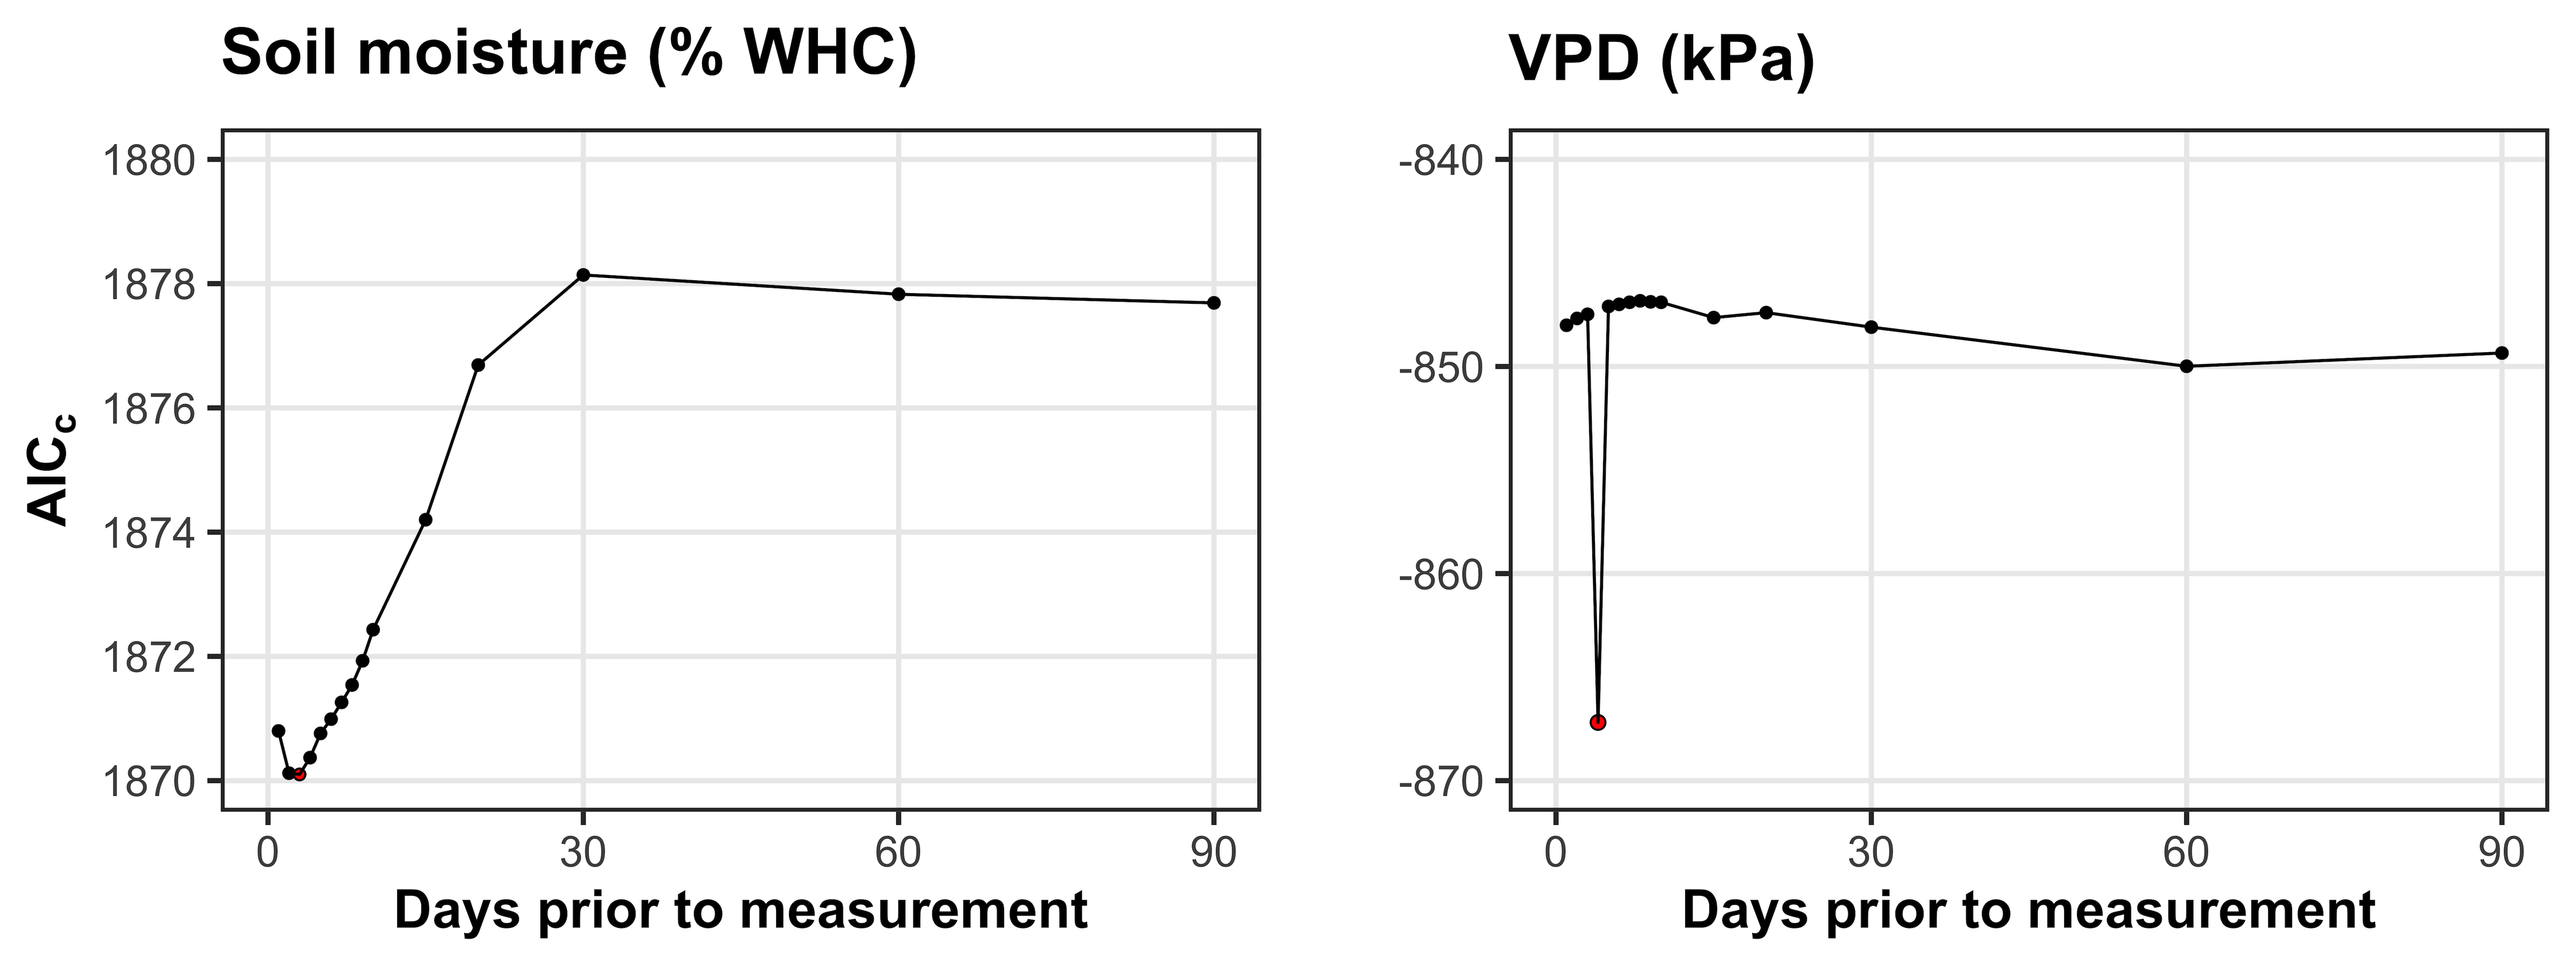
\includegraphics[width=\linewidth]{ch4_TXeco/figs/TXeco_figS2_aicc.jpg}
        \caption[Model selection results exploring relevant timescales for soil moisture and vapor pressure deficit]{Model selection results exploring relevant timescales for soil moisture (left panel) and vapor pressure deficit (right panel). The x-axis indicates the number of days before each site visit and the y-axis notes the corrected Akaike Information Criterion value. The timescale with the lowest AICc value, and therefore most relevant timescale to include in statistical models, is noted as a red point.}
        \label{fig:figure.c1}
    \end{figure}
\end{landscape}
\clearpage

